\subsection{Level3.1: パラメータのチューニング}
\subsubsection{最適なパラメータを探すためのアプローチ}
HIDDENとALPHAを固定してETAの最適な値を求め、その後にHIDDENとETAを固定してALPHAの最適な値を求める…というように、手動でのパラメータの探索を行った。

\subsubsection{実行結果}

\begin{table}[htb]
 \begin{center}
  \caption{階層型NNによる文字認識問題の学習に要した回数}
  \label{table:level3}
  \begin{tabular}[htb]{r|l} \hline
   シード値 & 収束した回数 \\ \hline \hline
   1000 & 62 \\ \hline
   2000 & 101 \\ \hline
   3000 & 101 \\ \hline
   4000 & 161 \\ \hline
   5000 & 75 \\ \hline
   6000 & 128 \\ \hline
   7000 & 71 \\ \hline
   8000 & 71 \\ \hline
   9000 & 58 \\ \hline
   10000 & 53 \\ \hline \hline
   10試行の平均値 & 88.1 \\ \hline
  \end{tabular}
 \end{center}
\end{table}

\begin{figure}[h]
 \begin{center}
  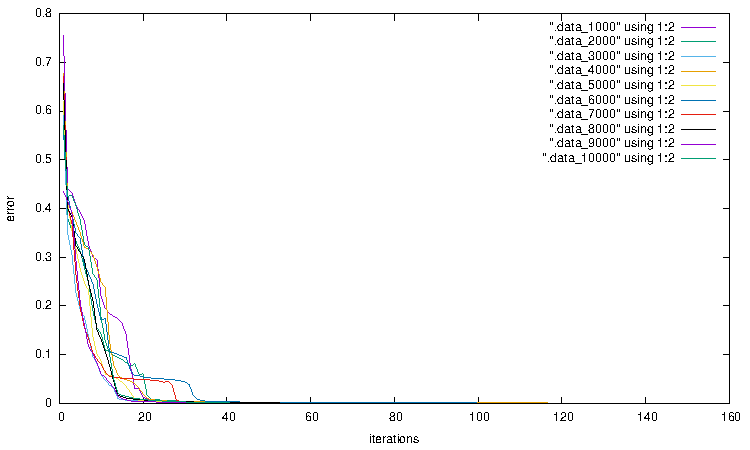
\includegraphics[width=10.0cm]{figs/level3.1/3_1.pdf}
  \caption{学習曲線}
  \label{fig:level3}
 \end{center}
\end{figure}


